\documentclass[1p]{elsarticle_modified}
%\bibliographystyle{elsarticle-num}

%\usepackage[colorlinks]{hyperref}
%\usepackage{abbrmath_seonhwa} %\Abb, \Ascr, \Acal ,\Abf, \Afrak
\usepackage{amsfonts}
\usepackage{amssymb}
\usepackage{amsmath}
\usepackage{amsthm}
\usepackage{scalefnt}
\usepackage{amsbsy}
\usepackage{kotex}
\usepackage{caption}
\usepackage{subfig}
\usepackage{color}
\usepackage{graphicx}
\usepackage{xcolor} %% white, black, red, green, blue, cyan, magenta, yellow
\usepackage{float}
\usepackage{setspace}
\usepackage{hyperref}

\usepackage{tikz}
\usetikzlibrary{arrows}

\usepackage{multirow}
\usepackage{array} % fixed length table
\usepackage{hhline}

%%%%%%%%%%%%%%%%%%%%%
\makeatletter
\renewcommand*\env@matrix[1][\arraystretch]{%
	\edef\arraystretch{#1}%
	\hskip -\arraycolsep
	\let\@ifnextchar\new@ifnextchar
	\array{*\c@MaxMatrixCols c}}
\makeatother %https://tex.stackexchange.com/questions/14071/how-can-i-increase-the-line-spacing-in-a-matrix
%%%%%%%%%%%%%%%

\usepackage[normalem]{ulem}

\newcommand{\msout}[1]{\ifmmode\text{\sout{\ensuremath{#1}}}\else\sout{#1}\fi}
%SOURCE: \msout is \stkout macro in https://tex.stackexchange.com/questions/20609/strikeout-in-math-mode

\newcommand{\cancel}[1]{
	\ifmmode
	{\color{red}\msout{#1}}
	\else
	{\color{red}\sout{#1}}
	\fi
}

\newcommand{\add}[1]{
	{\color{blue}\uwave{#1}}
}

\newcommand{\replace}[2]{
	\ifmmode
	{\color{red}\msout{#1}}{\color{blue}\uwave{#2}}
	\else
	{\color{red}\sout{#1}}{\color{blue}\uwave{#2}}
	\fi
}

\newcommand{\Sol}{\mathcal{S}} %segment
\newcommand{\D}{D} %diagram
\newcommand{\A}{\mathcal{A}} %arc


%%%%%%%%%%%%%%%%%%%%%%%%%%%%%5 test

\def\sl{\operatorname{\textup{SL}}(2,\Cbb)}
\def\psl{\operatorname{\textup{PSL}}(2,\Cbb)}
\def\quan{\mkern 1mu \triangleright \mkern 1mu}

\theoremstyle{definition}
\newtheorem{thm}{Theorem}[section]
\newtheorem{prop}[thm]{Proposition}
\newtheorem{lem}[thm]{Lemma}
\newtheorem{ques}[thm]{Question}
\newtheorem{cor}[thm]{Corollary}
\newtheorem{defn}[thm]{Definition}
\newtheorem{exam}[thm]{Example}
\newtheorem{rmk}[thm]{Remark}
\newtheorem{alg}[thm]{Algorithm}

\newcommand{\I}{\sqrt{-1}}
\begin{document}

%\begin{frontmatter}
%
%\title{Boundary parabolic representations of knots up to 8 crossings}
%
%%% Group authors per affiliation:
%\author{Yunhi Cho} 
%\address{Department of Mathematics, University of Seoul, Seoul, Korea}
%\ead{yhcho@uos.ac.kr}
%
%
%\author{Seonhwa Kim} %\fnref{s_kim}}
%\address{Center for Geometry and Physics, Institute for Basic Science, Pohang, 37673, Korea}
%\ead{ryeona17@ibs.re.kr}
%
%\author{Hyuk Kim}
%\address{Department of Mathematical Sciences, Seoul National University, Seoul 08826, Korea}
%\ead{hyukkim@snu.ac.kr}
%
%\author{Seokbeom Yoon}
%\address{Department of Mathematical Sciences, Seoul National University, Seoul, 08826,  Korea}
%\ead{sbyoon15@snu.ac.kr}
%
%\begin{abstract}
%We find all boundary parabolic representation of knots up to 8 crossings.
%
%\end{abstract}
%\begin{keyword}
%    \MSC[2010] 57M25 
%\end{keyword}
%
%\end{frontmatter}

%\linenumbers
%\tableofcontents
%
\newcommand\colored[1]{\textcolor{white}{\rule[-0.35ex]{0.8em}{1.4ex}}\kern-0.8em\color{red} #1}%
%\newcommand\colored[1]{\textcolor{white}{ #1}\kern-2.17ex	\textcolor{white}{ #1}\kern-1.81ex	\textcolor{white}{ #1}\kern-2.15ex\color{red}#1	}

{\Large $\underline{12a_{0776}~(K12a_{0776})}$}

\setlength{\tabcolsep}{10pt}
\renewcommand{\arraystretch}{1.6}
\vspace{1cm}\begin{tabular}{m{100pt}>{\centering\arraybackslash}m{274pt}}
\multirow{5}{120pt}{
	\centering
	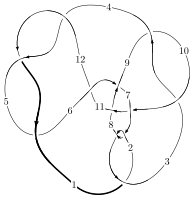
\includegraphics[width=112pt]{../../../GIT/diagram.site/Diagrams/png/1577_12a_0776.png}\\
\ \ \ A knot diagram\footnotemark}&
\allowdisplaybreaks
\textbf{Linearized knot diagam} \\
\cline{2-2}
 &
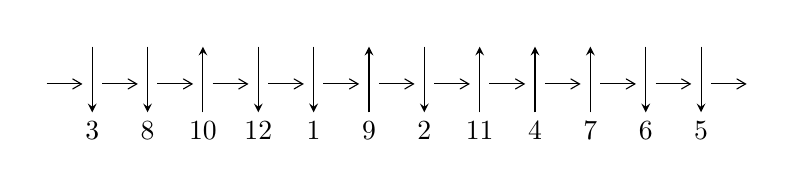
\begin{tikzpicture}[x=20pt, y=17pt]
	% nodes
	\node (C0) at (0, 0) {};
	\node (C1) at (1, 0) {};
	\node (C1U) at (1, +1) {};
	\node (C1D) at (1, -1) {3};

	\node (C2) at (2, 0) {};
	\node (C2U) at (2, +1) {};
	\node (C2D) at (2, -1) {8};

	\node (C3) at (3, 0) {};
	\node (C3U) at (3, +1) {};
	\node (C3D) at (3, -1) {10};

	\node (C4) at (4, 0) {};
	\node (C4U) at (4, +1) {};
	\node (C4D) at (4, -1) {12};

	\node (C5) at (5, 0) {};
	\node (C5U) at (5, +1) {};
	\node (C5D) at (5, -1) {1};

	\node (C6) at (6, 0) {};
	\node (C6U) at (6, +1) {};
	\node (C6D) at (6, -1) {9};

	\node (C7) at (7, 0) {};
	\node (C7U) at (7, +1) {};
	\node (C7D) at (7, -1) {2};

	\node (C8) at (8, 0) {};
	\node (C8U) at (8, +1) {};
	\node (C8D) at (8, -1) {11};

	\node (C9) at (9, 0) {};
	\node (C9U) at (9, +1) {};
	\node (C9D) at (9, -1) {4};

	\node (C10) at (10, 0) {};
	\node (C10U) at (10, +1) {};
	\node (C10D) at (10, -1) {7};

	\node (C11) at (11, 0) {};
	\node (C11U) at (11, +1) {};
	\node (C11D) at (11, -1) {6};

	\node (C12) at (12, 0) {};
	\node (C12U) at (12, +1) {};
	\node (C12D) at (12, -1) {5};
	\node (C13) at (13, 0) {};

	% arrows
	\draw[->,>={angle 60}]
	(C0) edge (C1) (C1) edge (C2) (C2) edge (C3) (C3) edge (C4) (C4) edge (C5) (C5) edge (C6) (C6) edge (C7) (C7) edge (C8) (C8) edge (C9) (C9) edge (C10) (C10) edge (C11) (C11) edge (C12) (C12) edge (C13) ;	\draw[->,>=stealth]
	(C1U) edge (C1D) (C2U) edge (C2D) (C3D) edge (C3U) (C4U) edge (C4D) (C5U) edge (C5D) (C6D) edge (C6U) (C7U) edge (C7D) (C8D) edge (C8U) (C9D) edge (C9U) (C10D) edge (C10U) (C11U) edge (C11D) (C12U) edge (C12D) ;
	\end{tikzpicture} \\
\hhline{~~} \\& 
\textbf{Solving Sequence} \\ \cline{2-2} 
 &
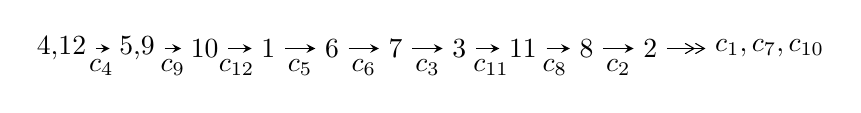
\begin{tikzpicture}[x=23pt, y=7pt]
	% node
	\node (A0) at (-1/8, 0) {4,12};
	\node (A1) at (17/16, 0) {5,9};
	\node (A2) at (17/8, 0) {10};
	\node (A3) at (25/8, 0) {1};
	\node (A4) at (33/8, 0) {6};
	\node (A5) at (41/8, 0) {7};
	\node (A6) at (49/8, 0) {3};
	\node (A7) at (57/8, 0) {11};
	\node (A8) at (65/8, 0) {8};
	\node (A9) at (73/8, 0) {2};
	\node (C1) at (1/2, -1) {$c_{4}$};
	\node (C2) at (13/8, -1) {$c_{9}$};
	\node (C3) at (21/8, -1) {$c_{12}$};
	\node (C4) at (29/8, -1) {$c_{5}$};
	\node (C5) at (37/8, -1) {$c_{6}$};
	\node (C6) at (45/8, -1) {$c_{3}$};
	\node (C7) at (53/8, -1) {$c_{11}$};
	\node (C8) at (61/8, -1) {$c_{8}$};
	\node (C9) at (69/8, -1) {$c_{2}$};
	\node (A10) at (11, 0) {$c_{1},c_{7},c_{10}$};

	% edge
	\draw[->,>=stealth]	
	(A0) edge (A1) (A1) edge (A2) (A2) edge (A3) (A3) edge (A4) (A4) edge (A5) (A5) edge (A6) (A6) edge (A7) (A7) edge (A8) (A8) edge (A9) ;
	\draw[->>,>={angle 60}]	
	(A9) edge (A10);
\end{tikzpicture} \\ 

\end{tabular} \\

\footnotetext{
The image of knot diagram is generated by the software ``\textbf{Draw programme}" developed by Andrew Bartholomew(\url{http://www.layer8.co.uk/maths/draw/index.htm\#Running-draw}), where we modified some parts for our purpose(\url{https://github.com/CATsTAILs/LinksPainter}).
}\phantom \\ \newline 
\centering \textbf{Ideals for irreducible components\footnotemark of $X_{\text{par}}$} 
 
\begin{align*}
I^u_{1}&=\langle 
6.98170\times10^{214} u^{129}+4.61169\times10^{214} u^{128}+\cdots+5.45825\times10^{214} b-8.94276\times10^{215},\\
\phantom{I^u_{1}}&\phantom{= \langle  }6.48861\times10^{215} u^{129}+6.31891\times10^{215} u^{128}+\cdots+1.03707\times10^{216} a+1.53636\times10^{215},\\
\phantom{I^u_{1}}&\phantom{= \langle  }u^{130}+2 u^{129}+\cdots+107 u-19\rangle \\
I^u_{2}&=\langle 
- u^{22}+11 u^{20}+\cdots+b+1,\;4 u^{22}+u^{21}+\cdots+a-6,\;u^{23}- u^{22}+\cdots- u+1\rangle \\
\\
\end{align*}
\raggedright * 2 irreducible components of $\dim_{\mathbb{C}}=0$, with total 153 representations.\\
\footnotetext{All coefficients of polynomials are rational numbers. But the coefficients are sometimes approximated in decimal forms when there is not enough margin.}
\newpage
\renewcommand{\arraystretch}{1}
\centering \section*{I. $I^u_{1}= \langle 6.98\times10^{214} u^{129}+4.61\times10^{214} u^{128}+\cdots+5.46\times10^{214} b-8.94\times10^{215},\;6.49\times10^{215} u^{129}+6.32\times10^{215} u^{128}+\cdots+1.04\times10^{216} a+1.54\times10^{215},\;u^{130}+2 u^{129}+\cdots+107 u-19 \rangle$}
\flushleft \textbf{(i) Arc colorings}\\
\begin{tabular}{m{7pt} m{180pt} m{7pt} m{180pt} }
\flushright $a_{4}=$&$\begin{pmatrix}1\\0\end{pmatrix}$ \\
\flushright $a_{12}=$&$\begin{pmatrix}0\\u\end{pmatrix}$ \\
\flushright $a_{5}=$&$\begin{pmatrix}1\\u^2\end{pmatrix}$ \\
\flushright $a_{9}=$&$\begin{pmatrix}-0.625668 u^{129}-0.609305 u^{128}+\cdots-27.4160 u-0.148144\\-1.27911 u^{129}-0.844901 u^{128}+\cdots-95.2397 u+16.3839\end{pmatrix}$ \\
\flushright $a_{10}=$&$\begin{pmatrix}-1.90478 u^{129}-1.45421 u^{128}+\cdots-122.656 u+16.2358\\-1.27911 u^{129}-0.844901 u^{128}+\cdots-95.2397 u+16.3839\end{pmatrix}$ \\
\flushright $a_{1}=$&$\begin{pmatrix}- u\\- u^3+u\end{pmatrix}$ \\
\flushright $a_{6}=$&$\begin{pmatrix}- u^2+1\\- u^4+2 u^2\end{pmatrix}$ \\
\flushright $a_{7}=$&$\begin{pmatrix}2.56893 u^{129}+2.78359 u^{128}+\cdots+230.909 u-39.9412\\0.412250 u^{129}+0.950242 u^{128}+\cdots+44.8273 u-6.37800\end{pmatrix}$ \\
\flushright $a_{3}=$&$\begin{pmatrix}3.56700 u^{129}+2.55922 u^{128}+\cdots+345.494 u-54.3475\\4.11991 u^{129}+3.15276 u^{128}+\cdots+415.557 u-63.9594\end{pmatrix}$ \\
\flushright $a_{11}=$&$\begin{pmatrix}u^5-2 u^3+u\\u^7-3 u^5+2 u^3+u\end{pmatrix}$ \\
\flushright $a_{8}=$&$\begin{pmatrix}-1.64224 u^{129}-0.895692 u^{128}+\cdots-84.3781 u+10.1577\\-1.83002 u^{129}-1.24918 u^{128}+\cdots-126.166 u+21.6069\end{pmatrix}$ \\
\flushright $a_{2}=$&$\begin{pmatrix}-3.81368 u^{129}-1.73033 u^{128}+\cdots-160.211 u+30.0156\\-2.52627 u^{129}-1.03451 u^{128}+\cdots-186.927 u+28.6906\end{pmatrix}$\\&\end{tabular}
\flushleft \textbf{(ii) Obstruction class $= -1$}\\~\\
\flushleft \textbf{(iii) Cusp Shapes $= 4.84806 u^{129}+2.00475 u^{128}+\cdots+371.144 u-52.0264$}\\~\\
\newpage\renewcommand{\arraystretch}{1}
\flushleft \textbf{(iv) u-Polynomials at the component}\newline \\
\begin{tabular}{m{50pt}|m{274pt}}
Crossings & \hspace{64pt}u-Polynomials at each crossing \\
\hline $$\begin{aligned}c_{1}\end{aligned}$$&$\begin{aligned}
&u^{130}+57 u^{129}+\cdots+113740 u+5776
\end{aligned}$\\
\hline $$\begin{aligned}c_{2},c_{7}\end{aligned}$$&$\begin{aligned}
&u^{130}+u^{129}+\cdots+90 u+76
\end{aligned}$\\
\hline $$\begin{aligned}c_{3},c_{9}\end{aligned}$$&$\begin{aligned}
&u^{130}+u^{129}+\cdots+7 u-1
\end{aligned}$\\
\hline $$\begin{aligned}c_{4},c_{5},c_{12}\end{aligned}$$&$\begin{aligned}
&u^{130}+2 u^{129}+\cdots+107 u-19
\end{aligned}$\\
\hline $$\begin{aligned}c_{6}\end{aligned}$$&$\begin{aligned}
&u^{130}+12 u^{129}+\cdots-270 u-19
\end{aligned}$\\
\hline $$\begin{aligned}c_{8}\end{aligned}$$&$\begin{aligned}
&u^{130}+18 u^{129}+\cdots-2103 u+1217
\end{aligned}$\\
\hline $$\begin{aligned}c_{10}\end{aligned}$$&$\begin{aligned}
&u^{130}+u^{129}+\cdots-49 u-1
\end{aligned}$\\
\hline $$\begin{aligned}c_{11}\end{aligned}$$&$\begin{aligned}
&u^{130}-6 u^{129}+\cdots+1396235 u-512411
\end{aligned}$\\
\hline
\end{tabular}\\~\\
\newpage\renewcommand{\arraystretch}{1}
\flushleft \textbf{(v) Riley Polynomials at the component}\newline \\
\begin{tabular}{m{50pt}|m{274pt}}
Crossings & \hspace{64pt}Riley Polynomials at each crossing \\
\hline $$\begin{aligned}c_{1}\end{aligned}$$&$\begin{aligned}
&y^{130}+43 y^{129}+\cdots-401377392 y+33362176
\end{aligned}$\\
\hline $$\begin{aligned}c_{2},c_{7}\end{aligned}$$&$\begin{aligned}
&y^{130}-57 y^{129}+\cdots-113740 y+5776
\end{aligned}$\\
\hline $$\begin{aligned}c_{3},c_{9}\end{aligned}$$&$\begin{aligned}
&y^{130}+87 y^{129}+\cdots+41 y+1
\end{aligned}$\\
\hline $$\begin{aligned}c_{4},c_{5},c_{12}\end{aligned}$$&$\begin{aligned}
&y^{130}-116 y^{129}+\cdots+4815 y+361
\end{aligned}$\\
\hline $$\begin{aligned}c_{6}\end{aligned}$$&$\begin{aligned}
&y^{130}+4 y^{129}+\cdots+53792 y+361
\end{aligned}$\\
\hline $$\begin{aligned}c_{8}\end{aligned}$$&$\begin{aligned}
&y^{130}-28 y^{129}+\cdots-151952217 y+1481089
\end{aligned}$\\
\hline $$\begin{aligned}c_{10}\end{aligned}$$&$\begin{aligned}
&y^{130}+y^{129}+\cdots-73 y+1
\end{aligned}$\\
\hline $$\begin{aligned}c_{11}\end{aligned}$$&$\begin{aligned}
&y^{130}+28 y^{129}+\cdots-9070292069281 y+262565032921
\end{aligned}$\\
\hline
\end{tabular}\\~\\
\newpage\flushleft \textbf{(vi) Complex Volumes and Cusp Shapes}
$$\begin{array}{c|c|c}  
\text{Solutions to }I^u_{1}& \I (\text{vol} + \sqrt{-1}CS) & \text{Cusp shape}\\
 \hline 
\begin{aligned}
u &= \phantom{-}0.858387 + 0.531211 I \\
a &= -0.000790 + 0.509860 I \\
b &= -0.582173 - 1.234630 I\end{aligned}
 & -1.99971 + 9.85947 I & \phantom{-0.000000 } 0 \\ \hline\begin{aligned}
u &= \phantom{-}0.858387 - 0.531211 I \\
a &= -0.000790 - 0.509860 I \\
b &= -0.582173 + 1.234630 I\end{aligned}
 & -1.99971 - 9.85947 I & \phantom{-0.000000 } 0 \\ \hline\begin{aligned}
u &= -0.898768 + 0.468623 I \\
a &= -0.081360 + 0.538066 I \\
b &= \phantom{-}0.521121 - 1.115890 I\end{aligned}
 & -0.11864 - 4.16240 I & \phantom{-0.000000 } 0 \\ \hline\begin{aligned}
u &= -0.898768 - 0.468623 I \\
a &= -0.081360 - 0.538066 I \\
b &= \phantom{-}0.521121 + 1.115890 I\end{aligned}
 & -0.11864 + 4.16240 I & \phantom{-0.000000 } 0 \\ \hline\begin{aligned}
u &= -0.083322 + 0.963348 I \\
a &= -0.084625 - 0.382231 I \\
b &= \phantom{-}0.037380 + 0.621768 I\end{aligned}
 & \phantom{-}2.83683 + 2.67689 I & \phantom{-0.000000 } 0 \\ \hline\begin{aligned}
u &= -0.083322 - 0.963348 I \\
a &= -0.084625 + 0.382231 I \\
b &= \phantom{-}0.037380 - 0.621768 I\end{aligned}
 & \phantom{-}2.83683 - 2.67689 I & \phantom{-0.000000 } 0 \\ \hline\begin{aligned}
u &= -1.004880 + 0.290209 I \\
a &= \phantom{-}0.865674 - 0.893082 I \\
b &= -1.030620 - 0.343395 I\end{aligned}
 & \phantom{-}0.91394 - 4.12561 I & \phantom{-0.000000 } 0 \\ \hline\begin{aligned}
u &= -1.004880 - 0.290209 I \\
a &= \phantom{-}0.865674 + 0.893082 I \\
b &= -1.030620 + 0.343395 I\end{aligned}
 & \phantom{-}0.91394 + 4.12561 I & \phantom{-0.000000 } 0 \\ \hline\begin{aligned}
u &= \phantom{-}0.420538 + 0.836988 I \\
a &= \phantom{-}0.873483 - 0.065030 I \\
b &= -0.284296 + 1.068210 I\end{aligned}
 & \phantom{-}0.87806 - 4.73563 I & \phantom{-0.000000 } 0 \\ \hline\begin{aligned}
u &= \phantom{-}0.420538 - 0.836988 I \\
a &= \phantom{-}0.873483 + 0.065030 I \\
b &= -0.284296 - 1.068210 I\end{aligned}
 & \phantom{-}0.87806 + 4.73563 I & \phantom{-0.000000 } 0\\
 \hline 
 \end{array}$$\newpage$$\begin{array}{c|c|c}  
\text{Solutions to }I^u_{1}& \I (\text{vol} + \sqrt{-1}CS) & \text{Cusp shape}\\
 \hline 
\begin{aligned}
u &= -0.335113 + 0.836804 I \\
a &= -0.931730 - 0.080138 I \\
b &= \phantom{-}0.441840 + 0.934661 I\end{aligned}
 & \phantom{-}1.33578 + 0.56403 I & \phantom{-0.000000 } 0 \\ \hline\begin{aligned}
u &= -0.335113 - 0.836804 I \\
a &= -0.931730 + 0.080138 I \\
b &= \phantom{-}0.441840 - 0.934661 I\end{aligned}
 & \phantom{-}1.33578 - 0.56403 I & \phantom{-0.000000 } 0 \\ \hline\begin{aligned}
u &= -1.10302\phantom{ +0.000000I} \\
a &= \phantom{-}0.775817\phantom{ +0.000000I} \\
b &= -0.789416\phantom{ +0.000000I}\end{aligned}
 & -1.76903\phantom{ +0.000000I} & \phantom{-0.000000 } 0 \\ \hline\begin{aligned}
u &= \phantom{-}0.285462 + 0.825901 I \\
a &= -1.81147 + 0.60588 I \\
b &= \phantom{-}0.64553 - 1.32946 I\end{aligned}
 & -0.1981 - 14.6031 I & \phantom{-0.000000 } 0 \\ \hline\begin{aligned}
u &= \phantom{-}0.285462 - 0.825901 I \\
a &= -1.81147 - 0.60588 I \\
b &= \phantom{-}0.64553 + 1.32946 I\end{aligned}
 & -0.1981 + 14.6031 I & \phantom{-0.000000 } 0 \\ \hline\begin{aligned}
u &= -0.987953 + 0.541065 I \\
a &= -0.571922 - 0.059134 I \\
b &= \phantom{-}0.266608 + 0.830546 I\end{aligned}
 & \phantom{-}0.09367 + 2.56827 I & \phantom{-0.000000 } 0 \\ \hline\begin{aligned}
u &= -0.987953 - 0.541065 I \\
a &= -0.571922 + 0.059134 I \\
b &= \phantom{-}0.266608 - 0.830546 I\end{aligned}
 & \phantom{-}0.09367 - 2.56827 I & \phantom{-0.000000 } 0 \\ \hline\begin{aligned}
u &= \phantom{-}0.541925 + 0.684342 I \\
a &= \phantom{-}0.652657 + 0.110887 I \\
b &= \phantom{-}0.166422 + 0.851085 I\end{aligned}
 & \phantom{-}0.333452 - 0.252683 I & \phantom{-0.000000 } 0 \\ \hline\begin{aligned}
u &= \phantom{-}0.541925 - 0.684342 I \\
a &= \phantom{-}0.652657 - 0.110887 I \\
b &= \phantom{-}0.166422 - 0.851085 I\end{aligned}
 & \phantom{-}0.333452 + 0.252683 I & \phantom{-0.000000 } 0 \\ \hline\begin{aligned}
u &= \phantom{-}1.102160 + 0.253758 I \\
a &= -1.066500 - 0.898377 I \\
b &= \phantom{-}0.851738 - 0.518125 I\end{aligned}
 & \phantom{-}1.86982 - 0.83103 I & \phantom{-0.000000 } 0\\
 \hline 
 \end{array}$$\newpage$$\begin{array}{c|c|c}  
\text{Solutions to }I^u_{1}& \I (\text{vol} + \sqrt{-1}CS) & \text{Cusp shape}\\
 \hline 
\begin{aligned}
u &= \phantom{-}1.102160 - 0.253758 I \\
a &= -1.066500 + 0.898377 I \\
b &= \phantom{-}0.851738 + 0.518125 I\end{aligned}
 & \phantom{-}1.86982 + 0.83103 I & \phantom{-0.000000 } 0 \\ \hline\begin{aligned}
u &= \phantom{-}1.136000 + 0.030176 I \\
a &= \phantom{-}0.981440 - 0.667637 I \\
b &= -0.042634 + 1.045810 I\end{aligned}
 & -6.23069 - 2.66080 I & \phantom{-0.000000 } 0 \\ \hline\begin{aligned}
u &= \phantom{-}1.136000 - 0.030176 I \\
a &= \phantom{-}0.981440 + 0.667637 I \\
b &= -0.042634 - 1.045810 I\end{aligned}
 & -6.23069 + 2.66080 I & \phantom{-0.000000 } 0 \\ \hline\begin{aligned}
u &= -0.251176 + 0.814299 I \\
a &= \phantom{-}1.79456 + 0.70713 I \\
b &= -0.610782 - 1.215540 I\end{aligned}
 & \phantom{-}1.91441 + 8.72257 I & \phantom{-0.000000 } 0 \\ \hline\begin{aligned}
u &= -0.251176 - 0.814299 I \\
a &= \phantom{-}1.79456 - 0.70713 I \\
b &= -0.610782 + 1.215540 I\end{aligned}
 & \phantom{-}1.91441 - 8.72257 I & \phantom{-0.000000 } 0 \\ \hline\begin{aligned}
u &= -0.037572 + 0.806192 I \\
a &= -0.399881 + 0.366390 I \\
b &= \phantom{-}0.291035 + 0.079569 I\end{aligned}
 & \phantom{-}2.95991 + 2.80966 I & \phantom{-0.000000 } 0 \\ \hline\begin{aligned}
u &= -0.037572 - 0.806192 I \\
a &= -0.399881 - 0.366390 I \\
b &= \phantom{-}0.291035 - 0.079569 I\end{aligned}
 & \phantom{-}2.95991 - 2.80966 I & \phantom{-0.000000 } 0 \\ \hline\begin{aligned}
u &= -0.647077 + 0.466955 I \\
a &= -0.221642 + 0.331704 I \\
b &= -0.496804 + 0.477870 I\end{aligned}
 & \phantom{-}0.13637 + 4.01955 I & \phantom{-0.000000 } 0 \\ \hline\begin{aligned}
u &= -0.647077 - 0.466955 I \\
a &= -0.221642 - 0.331704 I \\
b &= -0.496804 - 0.477870 I\end{aligned}
 & \phantom{-}0.13637 - 4.01955 I & \phantom{-0.000000 } 0 \\ \hline\begin{aligned}
u &= -0.183392 + 0.749630 I \\
a &= -1.87602 + 0.53667 I \\
b &= \phantom{-}1.255920 - 0.197610 I\end{aligned}
 & \phantom{-}3.40227 + 8.02397 I & \phantom{-0.000000 } 0. - 8.23743 I\\
 \hline 
 \end{array}$$\newpage$$\begin{array}{c|c|c}  
\text{Solutions to }I^u_{1}& \I (\text{vol} + \sqrt{-1}CS) & \text{Cusp shape}\\
 \hline 
\begin{aligned}
u &= -0.183392 - 0.749630 I \\
a &= -1.87602 - 0.53667 I \\
b &= \phantom{-}1.255920 + 0.197610 I\end{aligned}
 & \phantom{-}3.40227 - 8.02397 I & \phantom{-0.000000 -}0. + 8.23743 I \\ \hline\begin{aligned}
u &= -1.191740 + 0.311840 I \\
a &= \phantom{-}0.024118 + 1.067890 I \\
b &= \phantom{-}0.161195 - 0.679089 I\end{aligned}
 & -0.171796 + 0.563010 I & \phantom{-0.000000 } 0 \\ \hline\begin{aligned}
u &= -1.191740 - 0.311840 I \\
a &= \phantom{-}0.024118 - 1.067890 I \\
b &= \phantom{-}0.161195 + 0.679089 I\end{aligned}
 & -0.171796 - 0.563010 I & \phantom{-0.000000 } 0 \\ \hline\begin{aligned}
u &= -0.070853 + 0.764239 I \\
a &= \phantom{-}1.06562 + 1.55913 I \\
b &= -0.280012 - 0.707308 I\end{aligned}
 & \phantom{-}3.24360 + 3.35091 I & \phantom{-}6.53466 - 8.76240 I \\ \hline\begin{aligned}
u &= -0.070853 - 0.764239 I \\
a &= \phantom{-}1.06562 - 1.55913 I \\
b &= -0.280012 + 0.707308 I\end{aligned}
 & \phantom{-}3.24360 - 3.35091 I & \phantom{-}6.53466 + 8.76240 I \\ \hline\begin{aligned}
u &= \phantom{-}0.246615 + 0.720604 I \\
a &= -2.13436 + 0.83952 I \\
b &= \phantom{-}0.337598 - 1.206740 I\end{aligned}
 & -4.66475 - 5.87886 I & -6.12270 + 7.07846 I \\ \hline\begin{aligned}
u &= \phantom{-}0.246615 - 0.720604 I \\
a &= -2.13436 - 0.83952 I \\
b &= \phantom{-}0.337598 + 1.206740 I\end{aligned}
 & -4.66475 + 5.87886 I & -6.12270 - 7.07846 I \\ \hline\begin{aligned}
u &= \phantom{-}1.23931\phantom{ +0.000000I} \\
a &= -1.85412\phantom{ +0.000000I} \\
b &= \phantom{-}0.145370\phantom{ +0.000000I}\end{aligned}
 & -1.16737\phantom{ +0.000000I} & \phantom{-0.000000 } 0 \\ \hline\begin{aligned}
u &= \phantom{-}1.134870 + 0.535688 I \\
a &= \phantom{-}0.626428 + 0.107886 I \\
b &= -0.394333 + 0.864051 I\end{aligned}
 & -0.82512 - 7.90541 I & \phantom{-0.000000 } 0 \\ \hline\begin{aligned}
u &= \phantom{-}1.134870 - 0.535688 I \\
a &= \phantom{-}0.626428 - 0.107886 I \\
b &= -0.394333 - 0.864051 I\end{aligned}
 & -0.82512 + 7.90541 I & \phantom{-0.000000 } 0\\
 \hline 
 \end{array}$$\newpage$$\begin{array}{c|c|c}  
\text{Solutions to }I^u_{1}& \I (\text{vol} + \sqrt{-1}CS) & \text{Cusp shape}\\
 \hline 
\begin{aligned}
u &= \phantom{-}1.245080 + 0.173938 I \\
a &= \phantom{-}1.021120 - 0.397967 I \\
b &= -0.492548 - 1.109200 I\end{aligned}
 & -3.46073 + 3.05016 I & \phantom{-0.000000 } 0 \\ \hline\begin{aligned}
u &= \phantom{-}1.245080 - 0.173938 I \\
a &= \phantom{-}1.021120 + 0.397967 I \\
b &= -0.492548 + 1.109200 I\end{aligned}
 & -3.46073 - 3.05016 I & \phantom{-0.000000 } 0 \\ \hline\begin{aligned}
u &= \phantom{-}0.143744 + 0.721391 I \\
a &= \phantom{-}1.87656 + 0.52922 I \\
b &= -1.061160 - 0.341838 I\end{aligned}
 & \phantom{-}4.71433 - 2.79991 I & \phantom{-}3.67971 + 2.47559 I \\ \hline\begin{aligned}
u &= \phantom{-}0.143744 - 0.721391 I \\
a &= \phantom{-}1.87656 - 0.52922 I \\
b &= -1.061160 + 0.341838 I\end{aligned}
 & \phantom{-}4.71433 + 2.79991 I & \phantom{-}3.67971 - 2.47559 I \\ \hline\begin{aligned}
u &= \phantom{-}0.649728 + 0.327883 I \\
a &= \phantom{-}0.253720 + 0.133156 I \\
b &= -0.204354 - 1.251600 I\end{aligned}
 & -6.29212 + 2.13876 I & -10.09902 - 1.16229 I \\ \hline\begin{aligned}
u &= \phantom{-}0.649728 - 0.327883 I \\
a &= \phantom{-}0.253720 - 0.133156 I \\
b &= -0.204354 + 1.251600 I\end{aligned}
 & -6.29212 - 2.13876 I & -10.09902 + 1.16229 I \\ \hline\begin{aligned}
u &= -1.251240 + 0.302585 I \\
a &= \phantom{-}0.536351 + 0.071547 I \\
b &= -0.613211 - 0.091360 I\end{aligned}
 & -0.796656 + 1.165520 I & \phantom{-0.000000 } 0 \\ \hline\begin{aligned}
u &= -1.251240 - 0.302585 I \\
a &= \phantom{-}0.536351 - 0.071547 I \\
b &= -0.613211 + 0.091360 I\end{aligned}
 & -0.796656 - 1.165520 I & \phantom{-0.000000 } 0 \\ \hline\begin{aligned}
u &= -0.265715 + 0.657057 I \\
a &= -1.77184 + 0.24968 I \\
b &= \phantom{-}0.790079 + 0.494585 I\end{aligned}
 & -0.07306 + 2.71892 I & -4.07089 - 6.67892 I \\ \hline\begin{aligned}
u &= -0.265715 - 0.657057 I \\
a &= -1.77184 - 0.24968 I \\
b &= \phantom{-}0.790079 - 0.494585 I\end{aligned}
 & -0.07306 - 2.71892 I & -4.07089 + 6.67892 I\\
 \hline 
 \end{array}$$\newpage$$\begin{array}{c|c|c}  
\text{Solutions to }I^u_{1}& \I (\text{vol} + \sqrt{-1}CS) & \text{Cusp shape}\\
 \hline 
\begin{aligned}
u &= -1.289740 + 0.091959 I \\
a &= \phantom{-}0.487671 - 0.497441 I \\
b &= -0.919604 + 0.424918 I\end{aligned}
 & -2.79729 - 0.29925 I & \phantom{-0.000000 } 0 \\ \hline\begin{aligned}
u &= -1.289740 - 0.091959 I \\
a &= \phantom{-}0.487671 + 0.497441 I \\
b &= -0.919604 - 0.424918 I\end{aligned}
 & -2.79729 + 0.29925 I & \phantom{-0.000000 } 0 \\ \hline\begin{aligned}
u &= -1.286060 + 0.217213 I \\
a &= -0.942728 + 0.296382 I \\
b &= \phantom{-}0.602910 - 0.732975 I\end{aligned}
 & -1.14693 + 3.01047 I & \phantom{-0.000000 } 0 \\ \hline\begin{aligned}
u &= -1.286060 - 0.217213 I \\
a &= -0.942728 - 0.296382 I \\
b &= \phantom{-}0.602910 + 0.732975 I\end{aligned}
 & -1.14693 - 3.01047 I & \phantom{-0.000000 } 0 \\ \hline\begin{aligned}
u &= \phantom{-}1.297020 + 0.168197 I \\
a &= \phantom{-}0.803997 + 0.674909 I \\
b &= \phantom{-}0.06844 + 1.75600 I\end{aligned}
 & -7.43887 - 0.64726 I & \phantom{-0.000000 } 0 \\ \hline\begin{aligned}
u &= \phantom{-}1.297020 - 0.168197 I \\
a &= \phantom{-}0.803997 - 0.674909 I \\
b &= \phantom{-}0.06844 - 1.75600 I\end{aligned}
 & -7.43887 + 0.64726 I & \phantom{-0.000000 } 0 \\ \hline\begin{aligned}
u &= \phantom{-}1.314830 + 0.065784 I \\
a &= -0.432923 - 0.952214 I \\
b &= \phantom{-}1.027710 + 0.621020 I\end{aligned}
 & -4.97328 + 5.01201 I & \phantom{-0.000000 } 0 \\ \hline\begin{aligned}
u &= \phantom{-}1.314830 - 0.065784 I \\
a &= -0.432923 + 0.952214 I \\
b &= \phantom{-}1.027710 - 0.621020 I\end{aligned}
 & -4.97328 - 5.01201 I & \phantom{-0.000000 } 0 \\ \hline\begin{aligned}
u &= \phantom{-}1.309110 + 0.220391 I \\
a &= -1.69121 - 1.55482 I \\
b &= \phantom{-}0.272681 - 0.998474 I\end{aligned}
 & -1.34053 - 2.82972 I & \phantom{-0.000000 } 0 \\ \hline\begin{aligned}
u &= \phantom{-}1.309110 - 0.220391 I \\
a &= -1.69121 + 1.55482 I \\
b &= \phantom{-}0.272681 + 0.998474 I\end{aligned}
 & -1.34053 + 2.82972 I & \phantom{-0.000000 } 0\\
 \hline 
 \end{array}$$\newpage$$\begin{array}{c|c|c}  
\text{Solutions to }I^u_{1}& \I (\text{vol} + \sqrt{-1}CS) & \text{Cusp shape}\\
 \hline 
\begin{aligned}
u &= -0.226503 + 0.629720 I \\
a &= -1.82895 - 0.59609 I \\
b &= \phantom{-}0.595575 + 0.950772 I\end{aligned}
 & -0.17888 + 2.24153 I & -2.03920 - 4.83013 I \\ \hline\begin{aligned}
u &= -0.226503 - 0.629720 I \\
a &= -1.82895 + 0.59609 I \\
b &= \phantom{-}0.595575 - 0.950772 I\end{aligned}
 & -0.17888 - 2.24153 I & -2.03920 + 4.83013 I \\ \hline\begin{aligned}
u &= \phantom{-}1.309960 + 0.318270 I \\
a &= -1.308210 + 0.373986 I \\
b &= \phantom{-}0.402858 - 0.719122 I\end{aligned}
 & -1.07582 - 7.25709 I & \phantom{-0.000000 } 0 \\ \hline\begin{aligned}
u &= \phantom{-}1.309960 - 0.318270 I \\
a &= -1.308210 - 0.373986 I \\
b &= \phantom{-}0.402858 + 0.719122 I\end{aligned}
 & -1.07582 + 7.25709 I & \phantom{-0.000000 } 0 \\ \hline\begin{aligned}
u &= -1.338960 + 0.174442 I \\
a &= \phantom{-}2.24878 - 1.21891 I \\
b &= -0.024251 - 0.916418 I\end{aligned}
 & -5.56464 - 2.29092 I & \phantom{-0.000000 } 0 \\ \hline\begin{aligned}
u &= -1.338960 - 0.174442 I \\
a &= \phantom{-}2.24878 + 1.21891 I \\
b &= -0.024251 + 0.916418 I\end{aligned}
 & -5.56464 + 2.29092 I & \phantom{-0.000000 } 0 \\ \hline\begin{aligned}
u &= -1.340680 + 0.210493 I \\
a &= -0.877607 + 0.528762 I \\
b &= -0.30500 + 1.81718 I\end{aligned}
 & -8.12771 + 4.44289 I & \phantom{-0.000000 } 0 \\ \hline\begin{aligned}
u &= -1.340680 - 0.210493 I \\
a &= -0.877607 - 0.528762 I \\
b &= -0.30500 - 1.81718 I\end{aligned}
 & -8.12771 - 4.44289 I & \phantom{-0.000000 } 0 \\ \hline\begin{aligned}
u &= \phantom{-}1.318240 + 0.347178 I \\
a &= -0.302737 + 0.449145 I \\
b &= \phantom{-}0.0350078 - 0.1026420 I\end{aligned}
 & -1.33416 - 6.99228 I & \phantom{-0.000000 } 0 \\ \hline\begin{aligned}
u &= \phantom{-}1.318240 - 0.347178 I \\
a &= -0.302737 - 0.449145 I \\
b &= \phantom{-}0.0350078 + 0.1026420 I\end{aligned}
 & -1.33416 + 6.99228 I & \phantom{-0.000000 } 0\\
 \hline 
 \end{array}$$\newpage$$\begin{array}{c|c|c}  
\text{Solutions to }I^u_{1}& \I (\text{vol} + \sqrt{-1}CS) & \text{Cusp shape}\\
 \hline 
\begin{aligned}
u &= -1.342730 + 0.240858 I \\
a &= \phantom{-}1.20491 - 1.89788 I \\
b &= -0.256076 - 1.209960 I\end{aligned}
 & -4.66530 + 8.85846 I & \phantom{-0.000000 } 0 \\ \hline\begin{aligned}
u &= -1.342730 - 0.240858 I \\
a &= \phantom{-}1.20491 + 1.89788 I \\
b &= -0.256076 + 1.209960 I\end{aligned}
 & -4.66530 - 8.85846 I & \phantom{-0.000000 } 0 \\ \hline\begin{aligned}
u &= -1.349190 + 0.211300 I \\
a &= -1.83931 + 0.52479 I \\
b &= \phantom{-}0.57970 + 1.46511 I\end{aligned}
 & -8.08214 + 2.22669 I & \phantom{-0.000000 } 0 \\ \hline\begin{aligned}
u &= -1.349190 - 0.211300 I \\
a &= -1.83931 - 0.52479 I \\
b &= \phantom{-}0.57970 - 1.46511 I\end{aligned}
 & -8.08214 - 2.22669 I & \phantom{-0.000000 } 0 \\ \hline\begin{aligned}
u &= \phantom{-}0.277760 + 0.559975 I \\
a &= \phantom{-}2.75484 - 0.37789 I \\
b &= -0.83736 + 1.18337 I\end{aligned}
 & -2.26658 - 6.27963 I & -6.34357 + 11.22337 I \\ \hline\begin{aligned}
u &= \phantom{-}0.277760 - 0.559975 I \\
a &= \phantom{-}2.75484 + 0.37789 I \\
b &= -0.83736 - 1.18337 I\end{aligned}
 & -2.26658 + 6.27963 I & -6.34357 - 11.22337 I \\ \hline\begin{aligned}
u &= \phantom{-}1.371230 + 0.136561 I \\
a &= \phantom{-}0.096261 - 0.232470 I \\
b &= \phantom{-}0.629399 + 0.641989 I\end{aligned}
 & -6.90132 - 2.06770 I & \phantom{-0.000000 } 0 \\ \hline\begin{aligned}
u &= \phantom{-}1.371230 - 0.136561 I \\
a &= \phantom{-}0.096261 + 0.232470 I \\
b &= \phantom{-}0.629399 - 0.641989 I\end{aligned}
 & -6.90132 + 2.06770 I & \phantom{-0.000000 } 0 \\ \hline\begin{aligned}
u &= -1.350410 + 0.292276 I \\
a &= -0.574263 + 0.744951 I \\
b &= \phantom{-}1.203480 - 0.246195 I\end{aligned}
 & -0.00337 + 6.46781 I & \phantom{-0.000000 } 0 \\ \hline\begin{aligned}
u &= -1.350410 - 0.292276 I \\
a &= -0.574263 - 0.744951 I \\
b &= \phantom{-}1.203480 + 0.246195 I\end{aligned}
 & -0.00337 - 6.46781 I & \phantom{-0.000000 } 0\\
 \hline 
 \end{array}$$\newpage$$\begin{array}{c|c|c}  
\text{Solutions to }I^u_{1}& \I (\text{vol} + \sqrt{-1}CS) & \text{Cusp shape}\\
 \hline 
\begin{aligned}
u &= \phantom{-}0.109627 + 0.601306 I \\
a &= -2.02450 - 0.50174 I \\
b &= \phantom{-}0.351609 - 1.133120 I\end{aligned}
 & -0.05515 - 5.77718 I & \phantom{-}2.75164 + 8.40546 I \\ \hline\begin{aligned}
u &= \phantom{-}0.109627 - 0.601306 I \\
a &= -2.02450 + 0.50174 I \\
b &= \phantom{-}0.351609 + 1.133120 I\end{aligned}
 & -0.05515 + 5.77718 I & \phantom{-}2.75164 - 8.40546 I \\ \hline\begin{aligned}
u &= \phantom{-}1.374500 + 0.260783 I \\
a &= \phantom{-}1.36759 + 0.71622 I \\
b &= -0.653101 + 1.173240 I\end{aligned}
 & -5.24269 - 5.52378 I & \phantom{-0.000000 } 0 \\ \hline\begin{aligned}
u &= \phantom{-}1.374500 - 0.260783 I \\
a &= \phantom{-}1.36759 - 0.71622 I \\
b &= -0.653101 - 1.173240 I\end{aligned}
 & -5.24269 + 5.52378 I & \phantom{-0.000000 } 0 \\ \hline\begin{aligned}
u &= -0.479566 + 0.355001 I \\
a &= -0.436840 - 0.693374 I \\
b &= -0.215840 + 0.910078 I\end{aligned}
 & -1.29796 + 0.90199 I & -5.18087 - 4.06045 I \\ \hline\begin{aligned}
u &= -0.479566 - 0.355001 I \\
a &= -0.436840 + 0.693374 I \\
b &= -0.215840 - 0.910078 I\end{aligned}
 & -1.29796 - 0.90199 I & -5.18087 + 4.06045 I \\ \hline\begin{aligned}
u &= \phantom{-}1.370910 + 0.305032 I \\
a &= \phantom{-}0.533182 + 0.876918 I \\
b &= -1.382640 - 0.102108 I\end{aligned}
 & -1.51815 - 11.83770 I & \phantom{-0.000000 } 0 \\ \hline\begin{aligned}
u &= \phantom{-}1.370910 - 0.305032 I \\
a &= \phantom{-}0.533182 - 0.876918 I \\
b &= -1.382640 + 0.102108 I\end{aligned}
 & -1.51815 + 11.83770 I & \phantom{-0.000000 } 0 \\ \hline\begin{aligned}
u &= -0.013333 + 0.592223 I \\
a &= \phantom{-}2.42975 + 0.29872 I \\
b &= -0.392539 - 0.807900 I\end{aligned}
 & \phantom{-}2.82904 - 0.08807 I & \phantom{-}5.60147 + 0.37026 I \\ \hline\begin{aligned}
u &= -0.013333 - 0.592223 I \\
a &= \phantom{-}2.42975 - 0.29872 I \\
b &= -0.392539 + 0.807900 I\end{aligned}
 & \phantom{-}2.82904 + 0.08807 I & \phantom{-}5.60147 - 0.37026 I\\
 \hline 
 \end{array}$$\newpage$$\begin{array}{c|c|c}  
\text{Solutions to }I^u_{1}& \I (\text{vol} + \sqrt{-1}CS) & \text{Cusp shape}\\
 \hline 
\begin{aligned}
u &= \phantom{-}1.397730 + 0.189525 I \\
a &= \phantom{-}0.958506 + 0.724031 I \\
b &= -0.177783 + 0.029116 I\end{aligned}
 & -5.89100 - 6.15905 I & \phantom{-0.000000 } 0 \\ \hline\begin{aligned}
u &= \phantom{-}1.397730 - 0.189525 I \\
a &= \phantom{-}0.958506 - 0.724031 I \\
b &= -0.177783 - 0.029116 I\end{aligned}
 & -5.89100 + 6.15905 I & \phantom{-0.000000 } 0 \\ \hline\begin{aligned}
u &= \phantom{-}0.362563 + 0.457638 I \\
a &= \phantom{-}0.208409 - 1.271840 I \\
b &= \phantom{-}0.569372 + 1.258850 I\end{aligned}
 & -2.66428 + 3.24443 I & -6.17705 - 2.02777 I \\ \hline\begin{aligned}
u &= \phantom{-}0.362563 - 0.457638 I \\
a &= \phantom{-}0.208409 + 1.271840 I \\
b &= \phantom{-}0.569372 - 1.258850 I\end{aligned}
 & -2.66428 - 3.24443 I & -6.17705 + 2.02777 I \\ \hline\begin{aligned}
u &= -1.39806 + 0.22871 I \\
a &= -1.58146 + 1.09204 I \\
b &= \phantom{-}0.94345 + 1.32751 I\end{aligned}
 & -7.59586 + 9.21921 I & \phantom{-0.000000 } 0 \\ \hline\begin{aligned}
u &= -1.39806 - 0.22871 I \\
a &= -1.58146 - 1.09204 I \\
b &= \phantom{-}0.94345 - 1.32751 I\end{aligned}
 & -7.59586 - 9.21921 I & \phantom{-0.000000 } 0 \\ \hline\begin{aligned}
u &= -1.40906 + 0.18020 I \\
a &= -0.736086 + 0.285567 I \\
b &= -0.55498 + 1.46645 I\end{aligned}
 & -8.27139 - 0.86389 I & \phantom{-0.000000 } 0 \\ \hline\begin{aligned}
u &= -1.40906 - 0.18020 I \\
a &= -0.736086 - 0.285567 I \\
b &= -0.55498 - 1.46645 I\end{aligned}
 & -8.27139 + 0.86389 I & \phantom{-0.000000 } 0 \\ \hline\begin{aligned}
u &= \phantom{-}1.41549 + 0.13332 I \\
a &= \phantom{-}0.418946 + 0.403074 I \\
b &= \phantom{-}0.214404 + 1.204350 I\end{aligned}
 & -7.22098 - 2.65469 I & \phantom{-0.000000 } 0 \\ \hline\begin{aligned}
u &= \phantom{-}1.41549 - 0.13332 I \\
a &= \phantom{-}0.418946 - 0.403074 I \\
b &= \phantom{-}0.214404 - 1.204350 I\end{aligned}
 & -7.22098 + 2.65469 I & \phantom{-0.000000 } 0\\
 \hline 
 \end{array}$$\newpage$$\begin{array}{c|c|c}  
\text{Solutions to }I^u_{1}& \I (\text{vol} + \sqrt{-1}CS) & \text{Cusp shape}\\
 \hline 
\begin{aligned}
u &= -1.39810 + 0.29350 I \\
a &= \phantom{-}1.93006 - 0.63919 I \\
b &= -0.405049 - 1.248080 I\end{aligned}
 & -9.89266 + 9.57242 I & \phantom{-0.000000 } 0 \\ \hline\begin{aligned}
u &= -1.39810 - 0.29350 I \\
a &= \phantom{-}1.93006 + 0.63919 I \\
b &= -0.405049 + 1.248080 I\end{aligned}
 & -9.89266 - 9.57242 I & \phantom{-0.000000 } 0 \\ \hline\begin{aligned}
u &= \phantom{-}1.40689 + 0.25940 I \\
a &= \phantom{-}1.025100 + 0.918783 I \\
b &= -0.815266 + 0.674857 I\end{aligned}
 & -5.41669 - 6.06942 I & \phantom{-0.000000 } 0 \\ \hline\begin{aligned}
u &= \phantom{-}1.40689 - 0.25940 I \\
a &= \phantom{-}1.025100 - 0.918783 I \\
b &= -0.815266 - 0.674857 I\end{aligned}
 & -5.41669 + 6.06942 I & \phantom{-0.000000 } 0 \\ \hline\begin{aligned}
u &= -0.486120 + 0.286145 I \\
a &= \phantom{-}0.185350 - 0.667609 I \\
b &= -0.568095 + 0.418020 I\end{aligned}
 & -1.31003 + 0.54175 I & -6.81683 - 1.31516 I \\ \hline\begin{aligned}
u &= -0.486120 - 0.286145 I \\
a &= \phantom{-}0.185350 + 0.667609 I \\
b &= -0.568095 - 0.418020 I\end{aligned}
 & -1.31003 - 0.54175 I & -6.81683 + 1.31516 I \\ \hline\begin{aligned}
u &= \phantom{-}0.133677 + 0.536129 I \\
a &= \phantom{-}2.10326 - 2.26270 I \\
b &= -0.392636 + 1.317170 I\end{aligned}
 & -3.37384 + 0.52133 I & -4.26987 + 2.66669 I \\ \hline\begin{aligned}
u &= \phantom{-}0.133677 - 0.536129 I \\
a &= \phantom{-}2.10326 + 2.26270 I \\
b &= -0.392636 - 1.317170 I\end{aligned}
 & -3.37384 - 0.52133 I & -4.26987 - 2.66669 I \\ \hline\begin{aligned}
u &= \phantom{-}1.41088 + 0.33302 I \\
a &= -1.59820 - 0.69108 I \\
b &= \phantom{-}0.63561 - 1.29752 I\end{aligned}
 & -3.36834 - 12.86740 I & \phantom{-0.000000 } 0 \\ \hline\begin{aligned}
u &= \phantom{-}1.41088 - 0.33302 I \\
a &= -1.59820 + 0.69108 I \\
b &= \phantom{-}0.63561 + 1.29752 I\end{aligned}
 & -3.36834 + 12.86740 I & \phantom{-0.000000 } 0\\
 \hline 
 \end{array}$$\newpage$$\begin{array}{c|c|c}  
\text{Solutions to }I^u_{1}& \I (\text{vol} + \sqrt{-1}CS) & \text{Cusp shape}\\
 \hline 
\begin{aligned}
u &= -1.45618 + 0.07653 I \\
a &= -0.039806 - 1.092760 I \\
b &= \phantom{-}0.212168 - 1.380370 I\end{aligned}
 & -12.94690 - 0.82105 I & \phantom{-0.000000 } 0 \\ \hline\begin{aligned}
u &= -1.45618 - 0.07653 I \\
a &= -0.039806 + 1.092760 I \\
b &= \phantom{-}0.212168 + 1.380370 I\end{aligned}
 & -12.94690 + 0.82105 I & \phantom{-0.000000 } 0 \\ \hline\begin{aligned}
u &= \phantom{-}1.42202 + 0.35852 I \\
a &= \phantom{-}0.998334 + 0.626365 I \\
b &= -0.413990 + 1.173780 I\end{aligned}
 & -4.21413 - 4.94470 I & \phantom{-0.000000 } 0 \\ \hline\begin{aligned}
u &= \phantom{-}1.42202 - 0.35852 I \\
a &= \phantom{-}0.998334 - 0.626365 I \\
b &= -0.413990 - 1.173780 I\end{aligned}
 & -4.21413 + 4.94470 I & \phantom{-0.000000 } 0 \\ \hline\begin{aligned}
u &= -1.42895 + 0.33404 I \\
a &= \phantom{-}1.58291 - 0.81065 I \\
b &= -0.65275 - 1.40414 I\end{aligned}
 & -5.6600 + 18.7966 I & \phantom{-0.000000 } 0 \\ \hline\begin{aligned}
u &= -1.42895 - 0.33404 I \\
a &= \phantom{-}1.58291 + 0.81065 I \\
b &= -0.65275 + 1.40414 I\end{aligned}
 & -5.6600 - 18.7966 I & \phantom{-0.000000 } 0 \\ \hline\begin{aligned}
u &= \phantom{-}0.076022 + 0.521366 I \\
a &= \phantom{-}0.08077 - 1.73568 I \\
b &= \phantom{-}0.15097 + 1.72552 I\end{aligned}
 & -3.58802 - 1.74131 I & -1.39572 + 5.92415 I \\ \hline\begin{aligned}
u &= \phantom{-}0.076022 - 0.521366 I \\
a &= \phantom{-}0.08077 + 1.73568 I \\
b &= \phantom{-}0.15097 - 1.72552 I\end{aligned}
 & -3.58802 + 1.74131 I & -1.39572 - 5.92415 I \\ \hline\begin{aligned}
u &= \phantom{-}1.49460 + 0.01515 I \\
a &= \phantom{-}0.054877 + 0.764810 I \\
b &= -0.241243 + 1.238930 I\end{aligned}
 & -8.21426 - 3.52836 I & \phantom{-0.000000 } 0 \\ \hline\begin{aligned}
u &= \phantom{-}1.49460 - 0.01515 I \\
a &= \phantom{-}0.054877 - 0.764810 I \\
b &= -0.241243 - 1.238930 I\end{aligned}
 & -8.21426 + 3.52836 I & \phantom{-0.000000 } 0\\
 \hline 
 \end{array}$$\newpage$$\begin{array}{c|c|c}  
\text{Solutions to }I^u_{1}& \I (\text{vol} + \sqrt{-1}CS) & \text{Cusp shape}\\
 \hline 
\begin{aligned}
u &= -1.48241 + 0.26739 I \\
a &= -1.011520 + 0.728457 I \\
b &= \phantom{-}0.054138 + 0.901494 I\end{aligned}
 & -6.09411 + 3.76031 I & \phantom{-0.000000 } 0 \\ \hline\begin{aligned}
u &= -1.48241 - 0.26739 I \\
a &= -1.011520 - 0.728457 I \\
b &= \phantom{-}0.054138 - 0.901494 I\end{aligned}
 & -6.09411 - 3.76031 I & \phantom{-0.000000 } 0 \\ \hline\begin{aligned}
u &= -1.47562 + 0.34827 I \\
a &= -0.982200 + 0.694474 I \\
b &= \phantom{-}0.264731 + 1.228100 I\end{aligned}
 & -5.16016 + 9.09654 I & \phantom{-0.000000 } 0 \\ \hline\begin{aligned}
u &= -1.47562 - 0.34827 I \\
a &= -0.982200 - 0.694474 I \\
b &= \phantom{-}0.264731 - 1.228100 I\end{aligned}
 & -5.16016 - 9.09654 I & \phantom{-0.000000 } 0 \\ \hline\begin{aligned}
u &= -1.54342 + 0.01292 I \\
a &= \phantom{-}0.097509 - 0.778763 I \\
b &= \phantom{-}0.356165 - 1.265910 I\end{aligned}
 & -10.29580 - 8.53203 I & \phantom{-0.000000 } 0 \\ \hline\begin{aligned}
u &= -1.54342 - 0.01292 I \\
a &= \phantom{-}0.097509 + 0.778763 I \\
b &= \phantom{-}0.356165 + 1.265910 I\end{aligned}
 & -10.29580 + 8.53203 I & \phantom{-0.000000 } 0 \\ \hline\begin{aligned}
u &= \phantom{-}0.076394 + 0.385183 I \\
a &= -3.85398 + 1.50660 I \\
b &= -0.219834 - 0.730621 I\end{aligned}
 & -1.02291 + 4.47699 I & -1.50211 - 1.73310 I \\ \hline\begin{aligned}
u &= \phantom{-}0.076394 - 0.385183 I \\
a &= -3.85398 - 1.50660 I \\
b &= -0.219834 + 0.730621 I\end{aligned}
 & -1.02291 - 4.47699 I & -1.50211 + 1.73310 I \\ \hline\begin{aligned}
u &= \phantom{-}0.221791 + 0.154271 I \\
a &= -1.16786 + 2.68312 I \\
b &= \phantom{-}0.406142 - 0.079977 I\end{aligned}
 & \phantom{-}1.50967 - 0.46289 I & \phantom{-}6.10398 - 0.66773 I \\ \hline\begin{aligned}
u &= \phantom{-}0.221791 - 0.154271 I \\
a &= -1.16786 - 2.68312 I \\
b &= \phantom{-}0.406142 + 0.079977 I\end{aligned}
 & \phantom{-}1.50967 + 0.46289 I & \phantom{-}6.10398 + 0.66773 I\\
 \hline 
 \end{array}$$\newpage\newpage\renewcommand{\arraystretch}{1}
\centering \section*{II. $I^u_{2}= \langle - u^{22}+11 u^{20}+\cdots+b+1,\;4 u^{22}+u^{21}+\cdots+a-6,\;u^{23}- u^{22}+\cdots- u+1 \rangle$}
\flushleft \textbf{(i) Arc colorings}\\
\begin{tabular}{m{7pt} m{180pt} m{7pt} m{180pt} }
\flushright $a_{4}=$&$\begin{pmatrix}1\\0\end{pmatrix}$ \\
\flushright $a_{12}=$&$\begin{pmatrix}0\\u\end{pmatrix}$ \\
\flushright $a_{5}=$&$\begin{pmatrix}1\\u^2\end{pmatrix}$ \\
\flushright $a_{9}=$&$\begin{pmatrix}-4 u^{22}- u^{21}+\cdots-11 u+6\\u^{22}-11 u^{20}+\cdots+5 u-1\end{pmatrix}$ \\
\flushright $a_{10}=$&$\begin{pmatrix}-3 u^{22}- u^{21}+\cdots-6 u+5\\u^{22}-11 u^{20}+\cdots+5 u-1\end{pmatrix}$ \\
\flushright $a_{1}=$&$\begin{pmatrix}- u\\- u^3+u\end{pmatrix}$ \\
\flushright $a_{6}=$&$\begin{pmatrix}- u^2+1\\- u^4+2 u^2\end{pmatrix}$ \\
\flushright $a_{7}=$&$\begin{pmatrix}2 u^{22}-19 u^{20}+\cdots-4 u-3\\- u^{22}+11 u^{20}+\cdots+7 u^2+2\end{pmatrix}$ \\
\flushright $a_{3}=$&$\begin{pmatrix}u^{22}- u^{21}+\cdots+10 u+3\\3 u^{22}-30 u^{20}+\cdots-2 u-4\end{pmatrix}$ \\
\flushright $a_{11}=$&$\begin{pmatrix}u^5-2 u^3+u\\u^7-3 u^5+2 u^3+u\end{pmatrix}$ \\
\flushright $a_{8}=$&$\begin{pmatrix}-6 u^{22}-3 u^{21}+\cdots-10 u+8\\- u^{22}-2 u^{21}+\cdots+5 u+1\end{pmatrix}$ \\
\flushright $a_{2}=$&$\begin{pmatrix}u^{19}+2 u^{18}+\cdots+2 u+4\\6 u^{22}+u^{21}+\cdots+4 u-7\end{pmatrix}$\\&\end{tabular}
\flushleft \textbf{(ii) Obstruction class $= 1$}\\~\\
\flushleft \textbf{(iii) Cusp Shapes $= u^{22}-5 u^{21}+3 u^{20}+46 u^{19}-73 u^{18}-181 u^{17}+312 u^{16}+403 u^{15}-562 u^{14}-569 u^{13}+326 u^{12}+517 u^{11}+332 u^{10}-226 u^9-544 u^8-79 u^7+201 u^6+115 u^5-45 u^4-10 u^3+67 u^2-6 u-3$}\\~\\
\newpage\renewcommand{\arraystretch}{1}
\flushleft \textbf{(iv) u-Polynomials at the component}\newline \\
\begin{tabular}{m{50pt}|m{274pt}}
Crossings & \hspace{64pt}u-Polynomials at each crossing \\
\hline $$\begin{aligned}c_{1}\end{aligned}$$&$\begin{aligned}
&u^{23}-12 u^{22}+\cdots+15 u-1
\end{aligned}$\\
\hline $$\begin{aligned}c_{2}\end{aligned}$$&$\begin{aligned}
&u^{23}-6 u^{21}+\cdots+u+1
\end{aligned}$\\
\hline $$\begin{aligned}c_{3}\end{aligned}$$&$\begin{aligned}
&u^{23}+12 u^{21}+\cdots+u+1
\end{aligned}$\\
\hline $$\begin{aligned}c_{4},c_{5}\end{aligned}$$&$\begin{aligned}
&u^{23}- u^{22}+\cdots- u+1
\end{aligned}$\\
\hline $$\begin{aligned}c_{6}\end{aligned}$$&$\begin{aligned}
&u^{23}- u^{22}+\cdots+2 u+1
\end{aligned}$\\
\hline $$\begin{aligned}c_{7}\end{aligned}$$&$\begin{aligned}
&u^{23}-6 u^{21}+\cdots+u-1
\end{aligned}$\\
\hline $$\begin{aligned}c_{8}\end{aligned}$$&$\begin{aligned}
&u^{23}- u^{22}+\cdots+11 u+1
\end{aligned}$\\
\hline $$\begin{aligned}c_{9}\end{aligned}$$&$\begin{aligned}
&u^{23}+12 u^{21}+\cdots+u-1
\end{aligned}$\\
\hline $$\begin{aligned}c_{10}\end{aligned}$$&$\begin{aligned}
&u^{23}-2 u^{22}+\cdots- u-1
\end{aligned}$\\
\hline $$\begin{aligned}c_{11}\end{aligned}$$&$\begin{aligned}
&u^{23}-3 u^{22}+\cdots+u+1
\end{aligned}$\\
\hline $$\begin{aligned}c_{12}\end{aligned}$$&$\begin{aligned}
&u^{23}+u^{22}+\cdots- u-1
\end{aligned}$\\
\hline
\end{tabular}\\~\\
\newpage\renewcommand{\arraystretch}{1}
\flushleft \textbf{(v) Riley Polynomials at the component}\newline \\
\begin{tabular}{m{50pt}|m{274pt}}
Crossings & \hspace{64pt}Riley Polynomials at each crossing \\
\hline $$\begin{aligned}c_{1}\end{aligned}$$&$\begin{aligned}
&y^{23}+8 y^{22}+\cdots+15 y-1
\end{aligned}$\\
\hline $$\begin{aligned}c_{2},c_{7}\end{aligned}$$&$\begin{aligned}
&y^{23}-12 y^{22}+\cdots+15 y-1
\end{aligned}$\\
\hline $$\begin{aligned}c_{3},c_{9}\end{aligned}$$&$\begin{aligned}
&y^{23}+24 y^{22}+\cdots-19 y-1
\end{aligned}$\\
\hline $$\begin{aligned}c_{4},c_{5},c_{12}\end{aligned}$$&$\begin{aligned}
&y^{23}-23 y^{22}+\cdots-17 y-1
\end{aligned}$\\
\hline $$\begin{aligned}c_{6}\end{aligned}$$&$\begin{aligned}
&y^{23}-3 y^{22}+\cdots+2 y-1
\end{aligned}$\\
\hline $$\begin{aligned}c_{8}\end{aligned}$$&$\begin{aligned}
&y^{23}-11 y^{22}+\cdots+11 y-1
\end{aligned}$\\
\hline $$\begin{aligned}c_{10}\end{aligned}$$&$\begin{aligned}
&y^{23}-2 y^{22}+\cdots+3 y-1
\end{aligned}$\\
\hline $$\begin{aligned}c_{11}\end{aligned}$$&$\begin{aligned}
&y^{23}+5 y^{22}+\cdots-13 y-1
\end{aligned}$\\
\hline
\end{tabular}\\~\\
\newpage\flushleft \textbf{(vi) Complex Volumes and Cusp Shapes}
$$\begin{array}{c|c|c}  
\text{Solutions to }I^u_{2}& \I (\text{vol} + \sqrt{-1}CS) & \text{Cusp shape}\\
 \hline 
\begin{aligned}
u &= -0.136765 + 0.886584 I \\
a &= -0.464886 - 0.768538 I \\
b &= \phantom{-}0.074383 + 0.711970 I\end{aligned}
 & \phantom{-}2.48459 + 2.92368 I & -5.95131 - 7.29773 I \\ \hline\begin{aligned}
u &= -0.136765 - 0.886584 I \\
a &= -0.464886 + 0.768538 I \\
b &= \phantom{-}0.074383 - 0.711970 I\end{aligned}
 & \phantom{-}2.48459 - 2.92368 I & -5.95131 + 7.29773 I \\ \hline\begin{aligned}
u &= -1.137400 + 0.237603 I \\
a &= \phantom{-}0.598332 - 0.648516 I \\
b &= -0.001655 + 0.543381 I\end{aligned}
 & -0.135533 + 1.181210 I & -0.14945 - 3.84915 I \\ \hline\begin{aligned}
u &= -1.137400 - 0.237603 I \\
a &= \phantom{-}0.598332 + 0.648516 I \\
b &= -0.001655 - 0.543381 I\end{aligned}
 & -0.135533 - 1.181210 I & -0.14945 + 3.84915 I \\ \hline\begin{aligned}
u &= -1.18937\phantom{ +0.000000I} \\
a &= \phantom{-}1.57849\phantom{ +0.000000I} \\
b &= -0.595455\phantom{ +0.000000I}\end{aligned}
 & -0.649623\phantom{ +0.000000I} & \phantom{-}4.33110\phantom{ +0.000000I} \\ \hline\begin{aligned}
u &= -0.464086 + 0.619189 I \\
a &= -0.780759 + 0.520096 I \\
b &= \phantom{-}0.322899 + 0.676984 I\end{aligned}
 & \phantom{-}0.86827 + 1.45338 I & \phantom{-}0.49234 - 5.72010 I \\ \hline\begin{aligned}
u &= -0.464086 - 0.619189 I \\
a &= -0.780759 - 0.520096 I \\
b &= \phantom{-}0.322899 - 0.676984 I\end{aligned}
 & \phantom{-}0.86827 - 1.45338 I & \phantom{-}0.49234 + 5.72010 I \\ \hline\begin{aligned}
u &= \phantom{-}1.260330 + 0.119748 I \\
a &= -1.46115 - 0.66855 I \\
b &= \phantom{-}0.525408 + 0.828935 I\end{aligned}
 & -4.41882 + 3.57519 I & -5.80927 - 5.34802 I \\ \hline\begin{aligned}
u &= \phantom{-}1.260330 - 0.119748 I \\
a &= -1.46115 + 0.66855 I \\
b &= \phantom{-}0.525408 - 0.828935 I\end{aligned}
 & -4.41882 - 3.57519 I & -5.80927 + 5.34802 I \\ \hline\begin{aligned}
u &= \phantom{-}1.280310 + 0.369130 I \\
a &= \phantom{-}0.577225 - 0.404945 I \\
b &= -0.234517 + 0.714938 I\end{aligned}
 & -1.81288 - 7.46568 I & -10.12623 + 9.56548 I\\
 \hline 
 \end{array}$$\newpage$$\begin{array}{c|c|c}  
\text{Solutions to }I^u_{2}& \I (\text{vol} + \sqrt{-1}CS) & \text{Cusp shape}\\
 \hline 
\begin{aligned}
u &= \phantom{-}1.280310 - 0.369130 I \\
a &= \phantom{-}0.577225 + 0.404945 I \\
b &= -0.234517 - 0.714938 I\end{aligned}
 & -1.81288 + 7.46568 I & -10.12623 - 9.56548 I \\ \hline\begin{aligned}
u &= \phantom{-}1.353890 + 0.130129 I \\
a &= \phantom{-}0.751565 + 0.094140 I \\
b &= \phantom{-}0.27703 + 1.62075 I\end{aligned}
 & -8.53828 - 2.94002 I & -13.49393 + 2.30648 I \\ \hline\begin{aligned}
u &= \phantom{-}1.353890 - 0.130129 I \\
a &= \phantom{-}0.751565 - 0.094140 I \\
b &= \phantom{-}0.27703 - 1.62075 I\end{aligned}
 & -8.53828 + 2.94002 I & -13.49393 - 2.30648 I \\ \hline\begin{aligned}
u &= -1.369740 + 0.143102 I \\
a &= -1.139000 + 0.741405 I \\
b &= -0.04448 + 1.63544 I\end{aligned}
 & -8.77933 + 0.50052 I & -12.97044 + 0.14608 I \\ \hline\begin{aligned}
u &= -1.369740 - 0.143102 I \\
a &= -1.139000 - 0.741405 I \\
b &= -0.04448 - 1.63544 I\end{aligned}
 & -8.77933 - 0.50052 I & -12.97044 - 0.14608 I \\ \hline\begin{aligned}
u &= -1.41992 + 0.22958 I \\
a &= -1.22821 + 1.25746 I \\
b &= \phantom{-}0.457852 + 1.150840 I\end{aligned}
 & -6.70083 + 8.08144 I & -8.35369 - 6.88540 I \\ \hline\begin{aligned}
u &= -1.41992 - 0.22958 I \\
a &= -1.22821 - 1.25746 I \\
b &= \phantom{-}0.457852 - 1.150840 I\end{aligned}
 & -6.70083 - 8.08144 I & -8.35369 + 6.88540 I \\ \hline\begin{aligned}
u &= \phantom{-}1.44924 + 0.28311 I \\
a &= \phantom{-}0.875266 + 0.848679 I \\
b &= -0.526388 + 0.943193 I\end{aligned}
 & -5.19446 - 4.96649 I & -7.36181 + 3.19745 I \\ \hline\begin{aligned}
u &= \phantom{-}1.44924 - 0.28311 I \\
a &= \phantom{-}0.875266 - 0.848679 I \\
b &= -0.526388 - 0.943193 I\end{aligned}
 & -5.19446 + 4.96649 I & -7.36181 - 3.19745 I \\ \hline\begin{aligned}
u &= \phantom{-}0.252157 + 0.442817 I \\
a &= \phantom{-}2.36364 + 1.41634 I \\
b &= -0.437807 + 0.961477 I\end{aligned}
 & -1.18000 - 5.38216 I & -3.42253 + 8.35444 I\\
 \hline 
 \end{array}$$\newpage$$\begin{array}{c|c|c}  
\text{Solutions to }I^u_{2}& \I (\text{vol} + \sqrt{-1}CS) & \text{Cusp shape}\\
 \hline 
\begin{aligned}
u &= \phantom{-}0.252157 - 0.442817 I \\
a &= \phantom{-}2.36364 - 1.41634 I \\
b &= -0.437807 - 0.961477 I\end{aligned}
 & -1.18000 + 5.38216 I & -3.42253 - 8.35444 I \\ \hline\begin{aligned}
u &= \phantom{-}0.026666 + 0.331345 I \\
a &= \phantom{-}1.61873 - 3.31404 I \\
b &= -0.11499 + 1.57789 I\end{aligned}
 & -4.10141 + 1.27066 I & -11.01927 + 0.35294 I \\ \hline\begin{aligned}
u &= \phantom{-}0.026666 - 0.331345 I \\
a &= \phantom{-}1.61873 + 3.31404 I \\
b &= -0.11499 - 1.57789 I\end{aligned}
 & -4.10141 - 1.27066 I & -11.01927 - 0.35294 I\\
 \hline 
 \end{array}$$\newpage
\newpage\renewcommand{\arraystretch}{1}
\centering \section*{ III. u-Polynomials}
\begin{tabular}{m{50pt}|m{274pt}}
Crossings & \hspace{64pt}u-Polynomials at each crossing \\
\hline $$\begin{aligned}c_{1}\end{aligned}$$&$\begin{aligned}
&(u^{23}-12 u^{22}+\cdots+15 u-1)(u^{130}+57 u^{129}+\cdots+113740 u+5776)
\end{aligned}$\\
\hline $$\begin{aligned}c_{2}\end{aligned}$$&$\begin{aligned}
&(u^{23}-6 u^{21}+\cdots+u+1)(u^{130}+u^{129}+\cdots+90 u+76)
\end{aligned}$\\
\hline $$\begin{aligned}c_{3}\end{aligned}$$&$\begin{aligned}
&(u^{23}+12 u^{21}+\cdots+u+1)(u^{130}+u^{129}+\cdots+7 u-1)
\end{aligned}$\\
\hline $$\begin{aligned}c_{4},c_{5}\end{aligned}$$&$\begin{aligned}
&(u^{23}- u^{22}+\cdots- u+1)(u^{130}+2 u^{129}+\cdots+107 u-19)
\end{aligned}$\\
\hline $$\begin{aligned}c_{6}\end{aligned}$$&$\begin{aligned}
&(u^{23}- u^{22}+\cdots+2 u+1)(u^{130}+12 u^{129}+\cdots-270 u-19)
\end{aligned}$\\
\hline $$\begin{aligned}c_{7}\end{aligned}$$&$\begin{aligned}
&(u^{23}-6 u^{21}+\cdots+u-1)(u^{130}+u^{129}+\cdots+90 u+76)
\end{aligned}$\\
\hline $$\begin{aligned}c_{8}\end{aligned}$$&$\begin{aligned}
&(u^{23}- u^{22}+\cdots+11 u+1)(u^{130}+18 u^{129}+\cdots-2103 u+1217)
\end{aligned}$\\
\hline $$\begin{aligned}c_{9}\end{aligned}$$&$\begin{aligned}
&(u^{23}+12 u^{21}+\cdots+u-1)(u^{130}+u^{129}+\cdots+7 u-1)
\end{aligned}$\\
\hline $$\begin{aligned}c_{10}\end{aligned}$$&$\begin{aligned}
&(u^{23}-2 u^{22}+\cdots- u-1)(u^{130}+u^{129}+\cdots-49 u-1)
\end{aligned}$\\
\hline $$\begin{aligned}c_{11}\end{aligned}$$&$\begin{aligned}
&(u^{23}-3 u^{22}+\cdots+u+1)(u^{130}-6 u^{129}+\cdots+1396235 u-512411)
\end{aligned}$\\
\hline $$\begin{aligned}c_{12}\end{aligned}$$&$\begin{aligned}
&(u^{23}+u^{22}+\cdots- u-1)(u^{130}+2 u^{129}+\cdots+107 u-19)
\end{aligned}$\\
\hline
\end{tabular}\newpage\renewcommand{\arraystretch}{1}
\centering \section*{ IV. Riley Polynomials}
\begin{tabular}{m{50pt}|m{274pt}}
Crossings & \hspace{64pt}Riley Polynomials at each crossing \\
\hline $$\begin{aligned}c_{1}\end{aligned}$$&$\begin{aligned}
&(y^{23}+8 y^{22}+\cdots+15 y-1)\\
&\cdot(y^{130}+43 y^{129}+\cdots-401377392 y+33362176)
\end{aligned}$\\
\hline $$\begin{aligned}c_{2},c_{7}\end{aligned}$$&$\begin{aligned}
&(y^{23}-12 y^{22}+\cdots+15 y-1)(y^{130}-57 y^{129}+\cdots-113740 y+5776)
\end{aligned}$\\
\hline $$\begin{aligned}c_{3},c_{9}\end{aligned}$$&$\begin{aligned}
&(y^{23}+24 y^{22}+\cdots-19 y-1)(y^{130}+87 y^{129}+\cdots+41 y+1)
\end{aligned}$\\
\hline $$\begin{aligned}c_{4},c_{5},c_{12}\end{aligned}$$&$\begin{aligned}
&(y^{23}-23 y^{22}+\cdots-17 y-1)(y^{130}-116 y^{129}+\cdots+4815 y+361)
\end{aligned}$\\
\hline $$\begin{aligned}c_{6}\end{aligned}$$&$\begin{aligned}
&(y^{23}-3 y^{22}+\cdots+2 y-1)(y^{130}+4 y^{129}+\cdots+53792 y+361)
\end{aligned}$\\
\hline $$\begin{aligned}c_{8}\end{aligned}$$&$\begin{aligned}
&(y^{23}-11 y^{22}+\cdots+11 y-1)\\
&\cdot(y^{130}-28 y^{129}+\cdots-151952217 y+1481089)
\end{aligned}$\\
\hline $$\begin{aligned}c_{10}\end{aligned}$$&$\begin{aligned}
&(y^{23}-2 y^{22}+\cdots+3 y-1)(y^{130}+y^{129}+\cdots-73 y+1)
\end{aligned}$\\
\hline $$\begin{aligned}c_{11}\end{aligned}$$&$\begin{aligned}
&(y^{23}+5 y^{22}+\cdots-13 y-1)\\
&\cdot(y^{130}+28 y^{129}+\cdots-9070292069281 y+262565032921)
\end{aligned}$\\
\hline
\end{tabular}
\vskip 2pc
\end{document}